\section{Programación orientada a objetos}
\subsection{Características de la \Poo}
La \lb{\Poo} (POO) es un paradigma de desarrollo de software. 
\begin{center}
	\begin{tikzpicture}
		\node[draw=lightblue, fill=lightblue!10, line width=1.5,text width=10cm] {Enfoque centrado en los conceptos (abstracciones) del dominio de aplicación $\longrightarrow$ \lb{\textbf{Objetos}}};
	\end{tikzpicture}
\end{center}
La etapa de \lb{modelado del programa} es fundamental
\begin{itemize}
	\item Identificar los objetos que requería la aplicación.
	\item Definir las relaciones entre dichos objetos.
	\item Utilizar un lenguaje formal para especificar los modelos.
\end{itemize}
\lb{Abstracción:} permite centrarnos en las propiedades de los tipos de datos y no en la implementación.

\lb{Modularidad:} permite descomponer el software en componentes (clases, funciones) que se pueden combinar para resolver el problema original.

\lb{Encapsulación:} permite agrupar en un mismo módilo tanto en la estructura como el comportamiento de los tipos de datos.

\lb{Ocultación de Información:} permite establecer la visibilidad de las propiedades de un módulo, diferenciando la parte pública y la parte privada.

\lb{Herencia:} permite definir unas clases a partir de otras.

\lb{Polimorfismo:} permite que una entidad pueda hacer referencia a objetos de diferente tipo en tiempo de ejecución. Relacionado con el concepto de \lb{ligadura dinámica}.
\subsection{Desarrollo orientado a objetos}
Identificar los \lb{objetos} relevantes al problema.

Describir los \lb{tipos de objetos} y su \lb{propiedades}.

Encontrar las \lb{operaciones} para los tipos de objetos.

Identificar \lb{relaciones} entre objetos.

Utilizar los tipos de objetos y relaciones para estructurar el software.
\begin{center}
	\fcolorbox{lightblue}{lightblue!10}{¿Cómo podemos formalizar el proceso?}
\end{center}
\subsection{UML}
\lb{U}nified \lb{M}odelling \lb{L}anguage

Lenguaje visual para el modelado de software.\\
Se basa en el uso de diagramas. Tipos:
\begin{itemize}
	\item \lb{Estructura:} Diferentes entidades que componen un programa.
	\item \lb{Comportamiento:} Respuesta que va a dar el programa y pasos para lograrlo.
\end{itemize}
Utilización:
\begin{itemize}
	\item Diagramas de \lb{clases}
	\item Diagramas de \lb{casos de uso}
	\item Diagramas de \lb{secuencia}
\end{itemize}
\subsection{Clases y Objetos}
Una \lb{clase} (concepto) es la definición de un \lb{objeto} (realización).
\begin{itemize}
	\item \lb{Nombre}
	\item \lb{Atributos} $\longrightarrow$ datos que definen su estado (clase/instancia).
	\item \lb{Métodos} $\longrightarrow$ funciones que implementa (clase/instancia).
\end{itemize}
\begin{center}
	\includegraphics{"Temas/Tema 2/screenshot001"}
\end{center}
\lb{Instanciación:} proceso mediante el cual se crea un objeto a partir de su clase.
\subsection{Encapsulación}
\subsubsection{Visibilidad}
La \lb{visibilidad} regula el acceso a la información dentro de una clase $\longrightarrow$ proceso de encapsulación.
\begin{itemize}
	\item \lb{Pública} (+) miembro accesible para las demás clases del programa.
	\item \lb{Protegida} (\#) miembro accesible sólo a las clases derivadas (herencia).
	\item \lb{Privada} (-) miembro sólo accesible por su clase.
\end{itemize}
\begin{center}
	\includegraphics{"Temas/Tema 2/screenshot002"}
\end{center}
\subsubsubsection{Caso de uso}
Se desea modelar mediante UML un supermercado en donde se tienen una serie de \lb{productos} (frescos, refrigerados, congelados y en conserva), guardados en \lb{almacenes}, y proporcionados por una serie de \lb{proveedores}.

Se desea también modelar los \lb{clientes} de dicho supermercado así como su \lb{cesta de la compra} y la forma en la que la llenan introduciendo productos.
\subsubsection{Dependencia}
Una \lb{dependencia} se establece cuando una clase o uno de sus miembros necesita de otra clase para funcionar.
\begin{itemize}
	\item Permite la libertad de elegir la estructura interna.
	\item Preserva el uso de externo de una clase durante su ciclo de vida
\end{itemize}
\begin{center}
	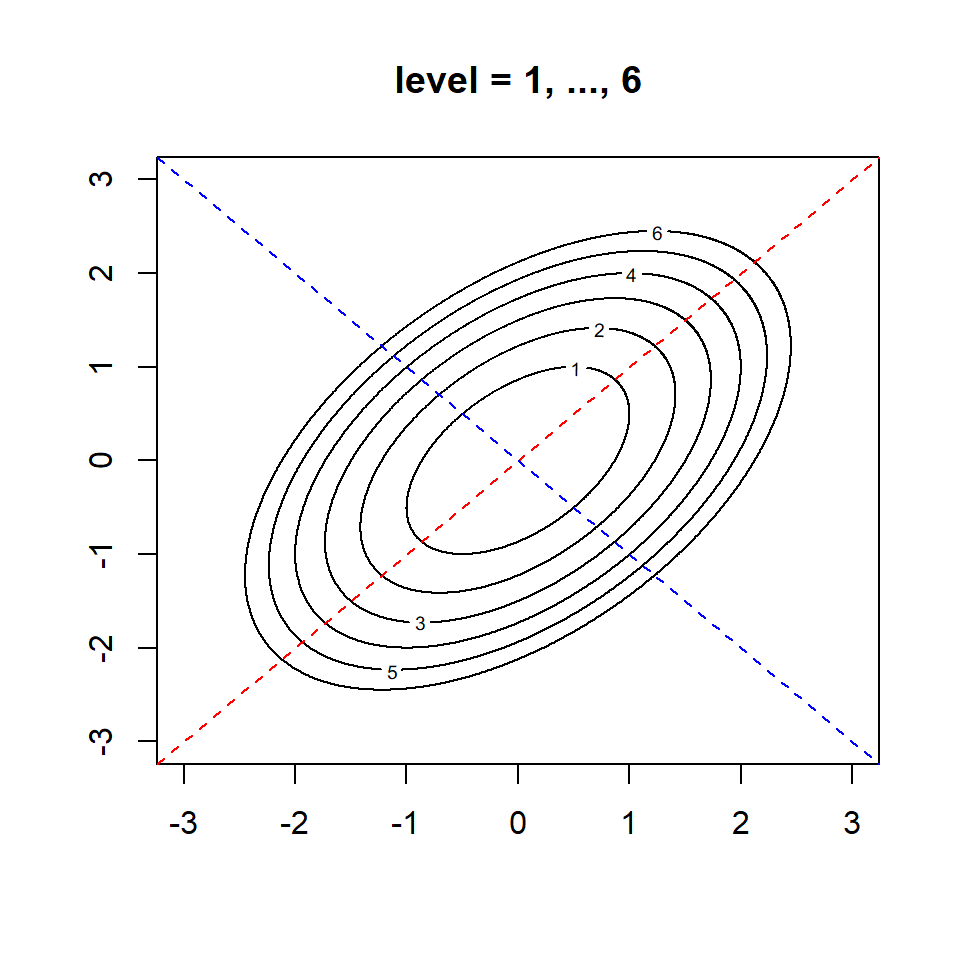
\includegraphics[width=0.5\linewidth]{"Temas/Tema 2/screenshot003.drawio"}
\end{center}
Gestión de las dependencias mediante \lb{visibilidad}.